\section{PNE Vigente} 

\subsection{Metas estabelecidas}

No Plano Nacional de Educação (2014-2024), a Meta 11 estabelecia o objetivo de triplicar as matrículas da Educação Profissional Técnica de Nível Médio (EPTNM) até 2024, assegurando que pelo menos 50\% da expansão ocorresse na rede pública. A tabela a seguir apresenta:
\begin{itemize}
	\item A meta definida para cada estado no PNE vigente;
	\item O total de matrículas de EPTNM registrado no Censo Escolar 2024;
	\item O déficit em relação à meta, a ser considerado para a elaboração do Plano de Aplicação de Recursos.
\end{itemize}

As matrículas de todas as redes de ensino foram consideradas nos dados a seguir. 

\begin{table}[!htbp] \centering 
	\caption{Meta 11 do PNE vs Matrículas Efetivas em EPTNM por Estado}
	\label{tab:meta11deficit}
	\footnotesize
	\begin{tabular}{@{\extracolsep{5pt}} lrrr} 
		\\[-1.8ex]\hline 
		\hline \\[-1.8ex] 
		Brasil e Estados & Meta 11 do PNE & Total de Matrículas de & Déficit de matrículas em \\
		& Matrículas em EPTNM & EPTNM (Censo, 2024) & relação à meta 11 \\ 
		\hline \\[-1.8ex] 
		Brasil & 4.614.621 & 2.352.083 & 2.262.538 \\ 
		Acre & 6.652 & 8.492 & - \\ 
		Alagoas & 42.507 & 24.589 & 17.918 \\ 
		Amapá & 15.903 & 5.605 & 10.298 \\ 
		Amazonas & 66.552 & 44.127 & 22.425 \\ 
		Bahia & 265.644 & 177.727 & 87.917 \\ 
		Ceará & 156.246 & 114.569 & 41.677 \\ 
		Distrito Federal & 45.342 & 30.053 & 15.289 \\ 
		Espírito Santo & 144.543 & 60.568 & 83.885 \\ 
		Goiás & 80.087 & 37.664 & 42.423 \\ 
		Maranhão & 76.029 & 71.075 & 4.924 \\ 
		Mato Grosso & 61.326 & 21.040 & 40.286 \\ 
		Mato Grosso do Sul & 61.821 & 20.928 & 40.893 \\ 
		Minas Gerais & 535.443 & 259.015 & 276.428 \\ 
		Pará & 77.283 & 61.194 & 16.089 \\ 
		Paraíba & 47.346 & 52.368 & - \\ 
		Paraná & 321.561 & 158.011 & 163.550 \\ 
		Pernambuco & 189.324 & 108.228 & 81.096 \\ 
		Piauí & 82.350 & 99.338 & - \\ 
		Rio de Janeiro & 489.018 & 146.789 & 342.229 \\ 
		Rio Grande do Norte & 69.348 & 55.628 & 13.720 \\ 
		Rio Grande do Sul & 314.736 & 138.757 & 175.979 \\ 
		Rondônia & 26.256 & 11.583 & 14.673 \\ 
		Roraima & 12.000 & 4.045 & 7.955 \\ 
		Santa Catarina & 197.310 & 82.602 & 114.708 \\ 
		São Paulo & 1.184.199 & 531.906 & 652.893 \\ 
		Sergipe & 13.386 & 15.532 & - \\ 
		Tocantins & 31.959 & 10.500 & 21.459 \\ 
		\hline \\[-1.8ex] 
	\end{tabular} 
\end{table}

No \textbf{Painel C1: PNE Vigente}, o gestor pode selecionar seu estado e visualizar a projeção do Ensino Médio e da EPTNM até 2035. Esse módulo foi desenhado para apoiar tecnicamente o desenvolvimento do Plano de Aplicação de Recursos pelos estados aderentes ao PROPAG, evidenciando a distância em relação à meta nacional e os desafios específicos de expansão. Além da opção de utilizar a Meta 11 estabelecida no PNE (2014–2024), o usuário também pode definir um valor alternativo de meta, de acordo com eventuais anúncios do MEC sobre os números oficiais de referência da Meta 11 para cada unidade da federação, que serão adotados no âmbito do PROPAG.



\begin{figure}[htbp!]
	\centering
	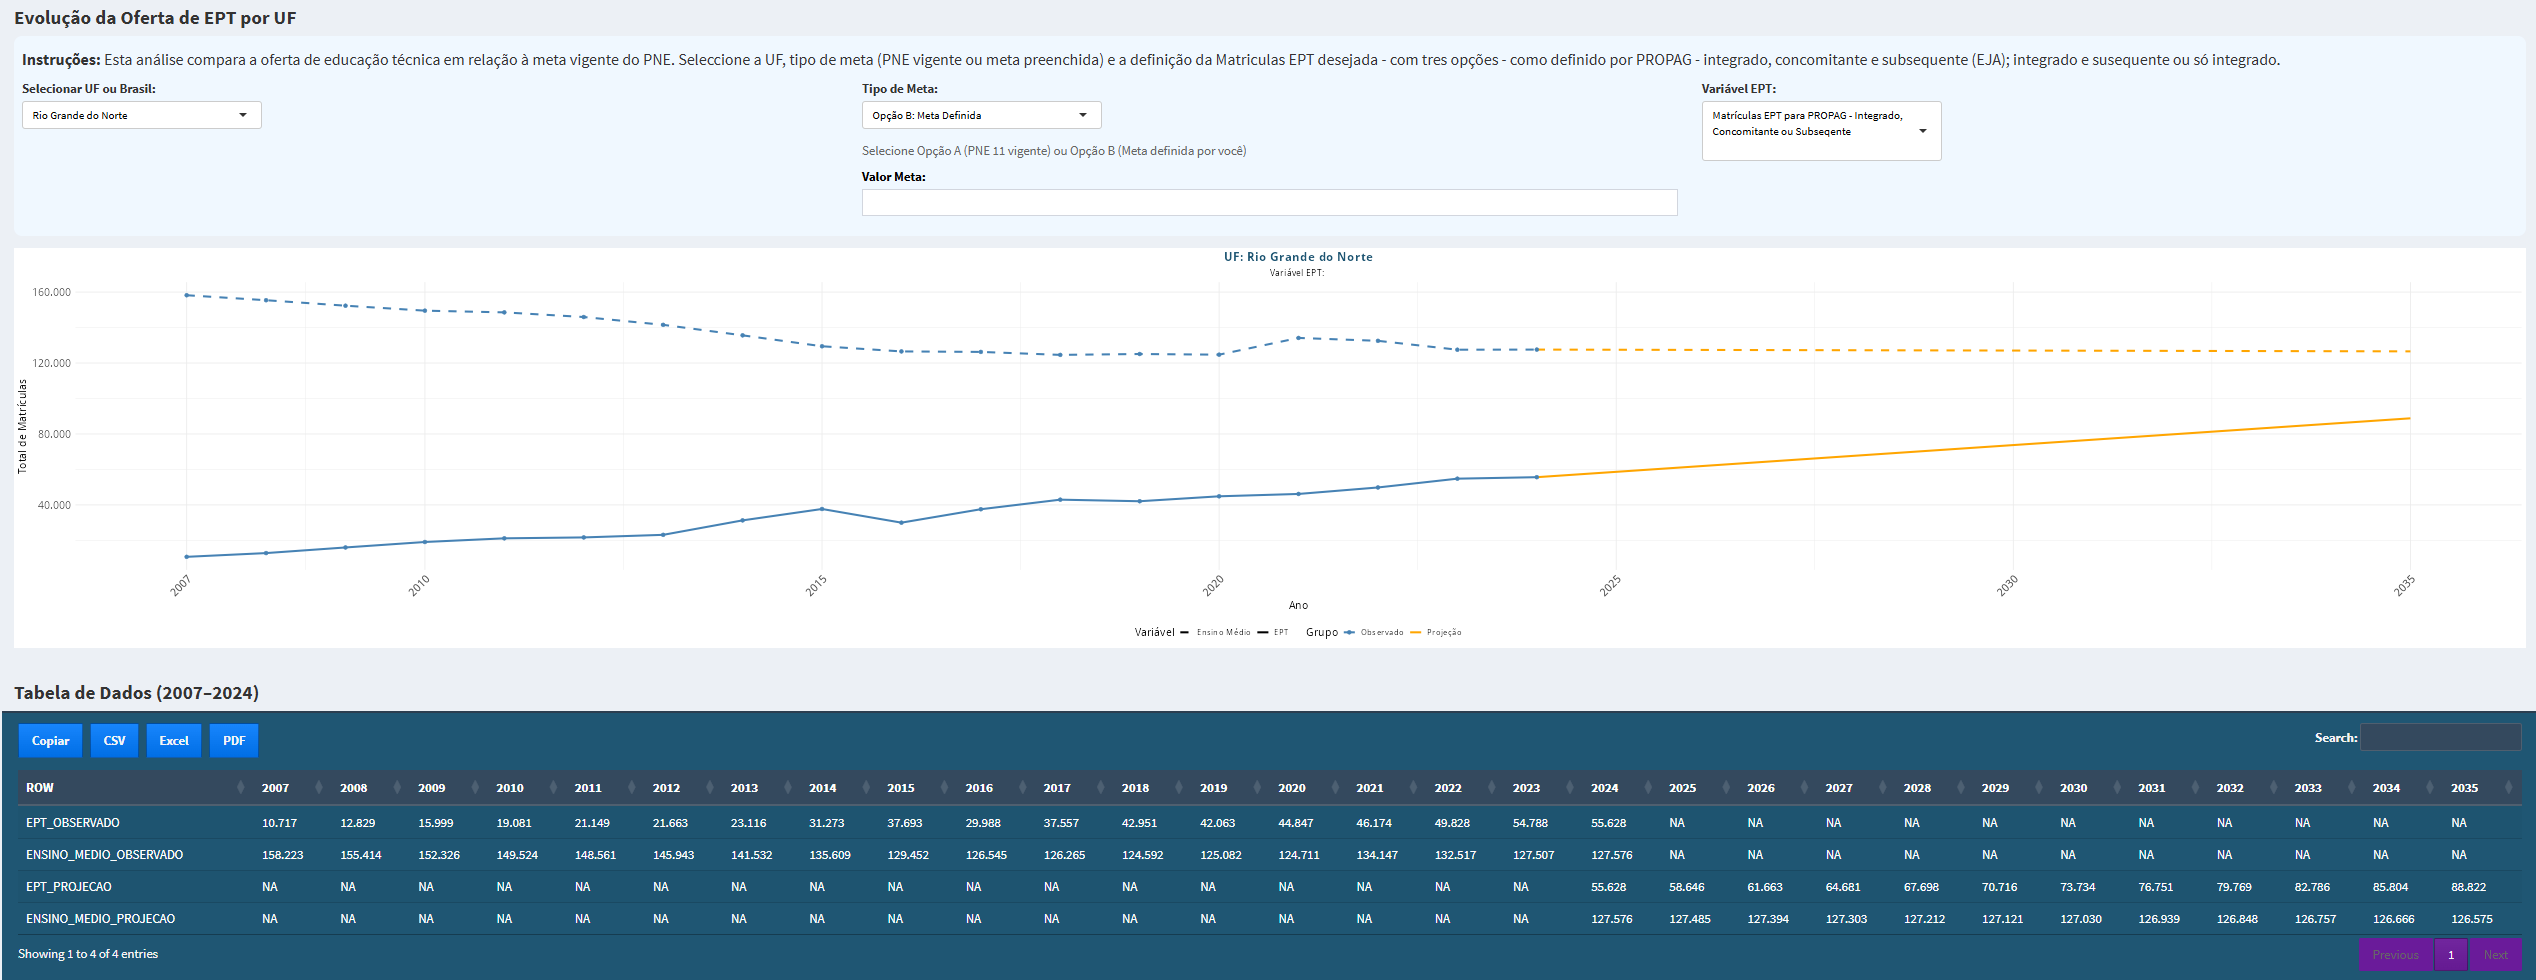
\includegraphics[width=1\textwidth]{images/TabC1_1a.png}
	\caption{Painel C1: Evolução da Oferta em relação à Meta 11 do PNE} 
	\label{fig:6a_Meta11}
\end{figure}

\subsection{Expansão das matrículas em EPT 2014-2024} 

Com base nos dados da Meta 11 do PNE, observa-se que o Brasil ainda está distante de alcançar a meta de 4,6 milhões de matrículas em EPTNM, registrando atualmente 2,35 milhões, com um déficit de 2,26 milhões de vagas. Estados populosos como São Paulo, Rio de Janeiro e Minas Gerais concentram a maior parte desse déficit, enquanto estados como Acre, Paraíba, Piauí e Sergipe já superaram a meta, indicando boas práticas locais que podem servir de referência. Há uma clara desigualdade regional: o Sudeste acumula o maior déficit absoluto, o Centro-Oeste apresenta lacunas proporcionais significativas, e o Nordeste mostra resultados mistos. 

Para atingir a meta, será necessário um crescimento acelerado e estratégico, priorizando estados com maior déficit absoluto e proporcional, ao mesmo tempo em que se aproveitam experiências bem-sucedidas em regiões que já superaram a meta. Essa constatação conduz diretamente à análise prospectiva apresentada no \textbf{Painel C2}, que permite comparar diferentes definições da Meta 11a, selecionar o ano-alvo para o seu cumprimento e calcular o incremento anual necessário de matrículas em cada cenário.


\section{PNE (2025–2035) na discussão}

\subsection{Política de Expansão da EPT}

Com a proximidade do encerramento do PNE 2014–2024 e a tramitação do novo PNE (2025–2035), o debate sobre a política de expansão da Educação Profissional Técnica de Nível Médio (EPTNM) torna-se central. O \textbf{Painel C2} foi desenvolvido para apoiar esse processo, permitindo que os gestores estaduais comparem diferentes definições da Meta 11a, selecionem o ano-alvo para o seu cumprimento e calculem o incremento anual necessário de matrículas em cada cenário.

A tabela a seguir organiza os principais elementos de análise:
\begin{itemize}
	\item O cenário atual das matrículas em EPTNM (Censo 2024);
	\item A projeção de matrículas no Ensino Médio em 2035;
	\item O aumento anual necessário de estudantes para atingir a meta;
	\item O percentual adicional de crescimento por ano até o ano-alvo.
\end{itemize}

Por fim, o painel contempla todas as redes de ensino e considera a EPTNM nas modalidades integrado, concomitante, subsequente e EJA, em conformidade com o escopo estabelecido para o PROPAG. O usuário pode ainda ajustar o crescimento projetado do Ensino Médio e simular diferentes horizontes de expansão, conforme a definição da meta utilizada pelo MEC ou valores alternativos adotados para o plano estadual.

\begin{figure}[htbp!]
	\centering
	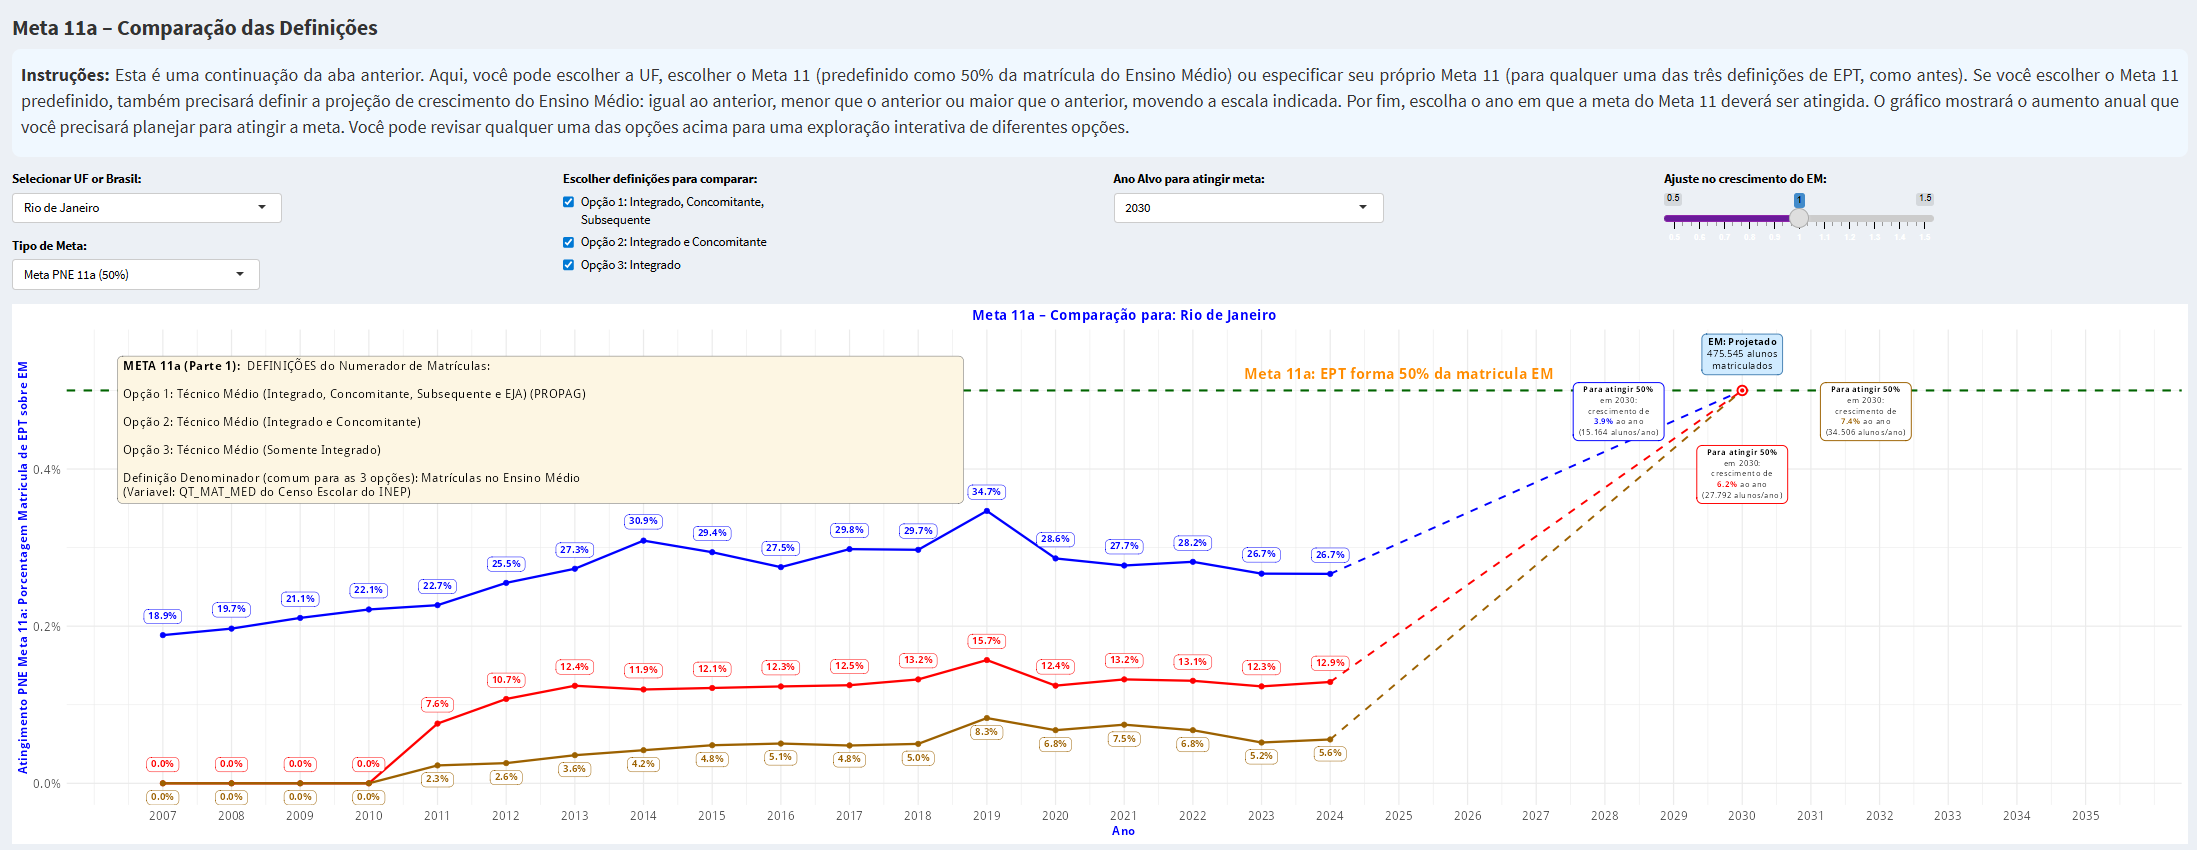
\includegraphics[width=1\textwidth]{images/TabC2_1a.png}
	\caption{Painel C2: Comparação das Definições da Meta 11a e Ano-Alvo}
	\label{fig:6b_Meta11a}
\end{figure}

\subsection{Trajetórias e Incrementos Necessários}

O Painel C2 mostra de forma interativa que a trajetória para o alcance da meta depende tanto da definição adotada para o numerador (todas as modalidades, apenas integrado e concomitante, ou apenas integrado) quanto do ano-alvo selecionado. Dessa forma, um estado pode planejar o ritmo de expansão em termos operacionais, expresso em \textit{novas matrículas por ano}, o que facilita a tradução da meta nacional em planos de ação estaduais.

Esse módulo complementa o diagnóstico do Painel C1: enquanto aquele evidencia o déficit atual frente à meta vigente, o Painel C2 oferece as alternativas de expansão para o próximo ciclo decenal de planejamento educacional, transformando o déficit em metas anuais concretas que podem ser incorporadas ao Plano de Aplicação de Recursos.


\section{Ampliação dos recursos para as redes}

Atingir os níveis de expansão projetados no \textbf{Painel C2} exige não apenas planejamento pedagógico, mas sobretudo capacidade financeira. A legislação do PROPAG estabelece que, até o cumprimento da Meta 11 do PNE, pelo menos 60\% dos recursos economizados com juros deverão ser aplicados em EPTNM. Isso significa que a sustentabilidade da trajetória até 2035 dependerá da articulação entre os investimentos constitucionais já realizados pelos estados, as transferências do Novo FUNDEB e os programas federais complementares.

As fontes de financiamento são essenciais para toda política pública, especialmente em um país com a complexidade geográfica, política, social e econômica como a do Brasil. A Educação Profissional precisa de recursos suficientes e estáveis, pois se trata de um processo contínuo, sustentado por professores, pesquisadores, estudantes e profissionais da educação em milhares de escolas distribuídas pelo território nacional.

A adesão ao PROPAG amplia os recursos disponíveis para todos os estados. Ao articular os valores obrigatórios de manutenção e desenvolvimento do ensino com os novos fatores de ponderação do FUNDEB e com programas federais como a Escola em Tempo Integral, os gestores estaduais poderão potencializar a capacidade de expansão e qualificação da oferta de EPT.

\subsection{Implicações do Novo FUNDEB}

Os novos Fatores de Ponderação nos Recursos do FUNDEB orientam a distribuição proporcional dos recursos, multiplicando o número de matrículas por coeficientes diferenciados. As modalidades da Formação Técnica Profissional (FTP) estão entre as mais valorizadas: 1,30 para o ensino médio articulado à educação profissional (curso técnico integrado), 1,40 para o ensino médio integral e 1,20 para a EJA integrada à educação profissional de nível médio. 

A Resolução nº 4, de 30 de outubro de 2023, especificou as diferenças e ponderações para o exercício de 2024, conforme a tabela abaixo:

\newenvironment{nomenclature}[1]
{
	\begin{table}[hbt]
		\caption{#1}
		\begin{center}
			\begin{tabular}{|l|l|l|}
				\hline
				\textbf{Symbol} & \textbf{Unit} & \textbf{Description}\\
				\hline
			}
			{
				\\\hline
			\end{tabular}
		\end{center}
	\end{table}
}

\begin{nomenclature}{Fatores de Ponderação FUNDEB - Resolução nº 4/2023}
	Ensino Médio Integral & 1,40 & um inteiro e quarenta centésimos\\
	Ensino Médio Articulado & 1,30 & um inteiro e trinta centésimos\\
	EJA Integrada EPT & 1,20 & um inteiro e vinte centésimos\\
	Formação Técnica & 1,30 & um inteiro e trinta centésimos
\end{nomenclature}

\subsection{Escola de Tempo Integral}

O Programa Escola em Tempo Integral, instituído pela Lei nº 14.640 de 2023, prevê a criação e ampliação de matrículas em tempo integral em todas as etapas e modalidades da educação básica. O programa assegura assistência técnica e financeira para matrículas com jornada mínima de sete horas diárias ou 35 horas semanais em dois turnos, priorizando estudantes em maior vulnerabilidade socioeconômica. 

As redes estaduais podem articular esse programa diretamente com a expansão da EPT, especialmente na modalidade do Ensino Médio Integrado com Curso Técnico (EMI) ou mesmo no formato concomitante em turnos complementares. Dessa forma, os recursos adicionais do programa não apenas aumentam o tempo de permanência escolar, mas também criam condições estruturais para ampliar a oferta de vagas técnicas em alinhamento com a Meta 11 do PNE.

\bigskip

Em síntese, os instrumentos financeiros — PROPAG, FUNDEB e Escola em Tempo Integral — constituem a base para transformar as trajetórias projetadas no Painel C2 em políticas exequíveis. A articulação entre esses mecanismos será decisiva para que cada unidade da federação consiga sustentar o crescimento anual de matrículas e reduzir as desigualdades regionais de acesso à EPT.
